Les techniques d'approximation d'EDPs d'évolution comportent souvent une étape nécessitant la résolution d'une équation différentielle ordinaire
\footnote{On utilisera aussi le terme \textit{système dynamique}, même si en toute rigueur ce concept est un peu plus large.} (EDO),
c'est à dire une équation différentielle ne faisant intervenir qu'une seule variable différenciée, généralement le temps. Cette section rappelle 
quelques notions d'analyse et de simulation des EDOs du premier ordre.\par

\begin{definition}[Équation différentielle ordinaire]
    Une équation différentielle ordinaire (du premier ordre) est une équation de la forme :
    \begin{align}\label{def:def_ODE}
        u' &= A(u,t)\quad u : t \in \mathbb{R}^+ \mapsto u(t) \in \mathbb{R}^d\\\notag
        u(0)&=u_0 \in \mathbb{R}^d.
    \end{align}
\end{definition}
%%%%%%%%%%%%%%%%%%%%%%%%%%%%%%%%%%%%%%%%%%%%%%%%%%%%%%%%%%%%%%%%%%%%%%%%    SCHEMA EXPLICITES ET IMPLICITES
\subsection{Schémas explicites et implicites.}
L'approximation des EDO se fait grâce à des schémas numériques, c'est à dire une suite d'élément $(u^n)$ de $\mathbb{R}^d$.
Donnés une EDO et un pas de discrétisation temporel $\Delta t$, $u^n \in \mathbb{R}^d$ est approxime la solution de l'EDO au temps $t^n = n \Delta t$.
C'est à dire que la suite $(u^n)_{n\in \mathbb{N}} \in (\mathbb R^d)^\mathbb{N}$ définie par un schéma numérique cherche à avoir à avoir $u^n \approx u(t=n\Delta t)$.
Deux catégories de schémas numériques existent: les schémas explicites et les schémas implicites
% Seuls les schémas à un pas sont ici présentés et non pas les schémas multi-pas. Ce choix est fait en raison de la barrière de Dahlquist
% \footnote{\url{https://fr.wikipedia.org/wiki/Methode_lineaire_a_pas_multiples\#Premiere_et_deuxieme_limites_de_Dahlquist}}.


\begin{definition}[Schéma explicite]
    Un schéma numérique est dit explicite si la solution au pas de temps $n+1$ est obtenu seulement grâce à la solution pas de temps $n$. Cela se formule usuellement sous la forme:
    \begin{align}
        u^{n+1} = u^n + f(u^n ,\Delta t ).
    \end{align}
\end{definition}

\begin{definition}[Schéma implicite]
    Un schéma numérique est dit implicite si la solution au pas  de temps $n+1$ est obtenue au moins en partie grâce à la solution pas de temps $n+1$. 
    Cela peut s'écrire écrit comme:
    \begin{align}
        u^{n+1} = u^n + f(u^{n+1} ,\Delta t ).
    \end{align}
    
\end{definition}

\textbf{Comparaison entre ces deux classes de schémas:}
Une itération d'un schéma implicite nécessite donc l'inversion d'un système linéaire ou non linéaire sur $\mathbb{R}^d$.
De fait, une itération implicite est généralement plus coûteuse qu'une itération d'un schéma explicite
\footnote{En particulier si la dimension de la solution $d$ est grande.}. 
Cependant pour des raisons de stabilités (voir \ref{par:stabilite_edo}) les méthodes explicites peuvent nécessiter des pas de temps bien plus fin, et donc bien plus d'itérations.
Le choix entre méthode explicite et implicite dépend de bien des facteurs (du problème, du niveau de précision voulu, de la difficulté d'implémentation etc...)
c'est un enjeu central de la simulation numérique.
%%%%%%%%%%%%%%%%%%%%%%%%%%%%%%%%%%%%%%%%%%%%%%%%%%%%%%%%%%%%%%%%%%%%%%%%
\subsection{Ordre de convergence d'un schéma}
L'ordre de convergence permet de lier l'erreur des solutions numérique au pas de temps, c'est-à-dire de quantifier l'efficacité d'un schéma numérique.
Pour définir la notion d'ordre de convergence d'un schéma numérique, il faut d'abord définir son erreur.
\begin{definition}[Erreur locale d'un schéma]
    L'erreur locale d'un schéma numérique de résolution d'une EDO est l'erreur que commet le schéma sur un pas de temps.
    Autrement dit si l'on note $u$ la solution de l'EDO à partir d'un état initial $u_0 = u(t=0)$ et $u_1$ l'approximation numérique proposée par la schéma 
    pour un pas de temps $\Delta t$ à partir de l'était $u_0$, l'erreur locale est: 
    \begin{align}
        e(\Delta t) = \Vert u(\Delta t) - u_1 \Vert_{\mathbb{R}^d}.
    \end{align}
\end{definition}

\begin{definition}[Erreur globale d'un schméa]
    L'erreur globale d'un schéma est l'erreur que commet le schéma sur plusieurs pas de temps. 
    Si l'on note $u^n$ la solution numérique au temps $t^n = n \Delta t$, alors l'erreur globale du schéma jusqu'au temps final $T = N \Delta t$ peut être définie comme:
    \begin{align}
        E(\Delta t) = \sum_{n=0}^N \Vert u^n - u(n^t) \Vert_{\mathbb{R}^d}
    \end{align}
    ou plus simplement encore:
    \begin{align}
        E(\Delta t)=\Vert u^n - u(T) \Vert_{\mathbb{R}^d}.
    \end{align}
\end{definition}

\begin{definition}[Ordre de convergence]
    Un schéma numérique de résolution d'une EDO est dit d'ordre $p$ si de manière équivalente:
    \begin{itemize}
        \item[$\diamond$] L'erreur locale vérifie : $e(\Delta t) = O(\Delta t^{p+1})$
        \item[$\diamond$] L'erreur globale vérifie : $E(\Delta t) = O(\Delta t^{p})$
    \end{itemize}
\end{definition}

%%%%%%%%%%%%%%%%%%%%%%%%%%%%%%%%%%%%%%%%%%%%%%%%%%%%%%%%%%%%%%%%%%%%%%%%


\subsection{Stabilité et raideur}\label{par:stabilite_edo}

Un schéma numérique d'ordre $p$ converge asymptotiquement en $O(\Delta t^p)$ vers la solution exacte d'une EDO lorsque $\Delta t$ est assez petit.
Cependant, cette convergence n'est effective que si le schéma est \textbf{stable}.  
Un schéma instable conduit à une divergence de la solution numérique : en pratique, au-delà d'un pas de temps critique $\Delta t_0$, la norme $\Vert u^n \Vert$ croît sans borne%
\footnote{Phénomène souvent appelé \og explosion numérique\fg.}, comme illustré figure~\ref{fig:stabilite_schema}.
Ainsi, pour entrer dans le régime asymptotique de convergence, il faut respecter une contrainte de stabilité de type $\Delta t \leq \Delta t_0$.  
Lorsque ce seuil est très faible, la simulation devient coûteuse car elle nécessite un grand nombre d’itérations $T_\mathrm{final}/\Delta t$.  
De manière générale, les schémas explicites sont plus sensibles à ces contraintes que les schémas implicites.

\begin{figure}[htbp]
    \centering
    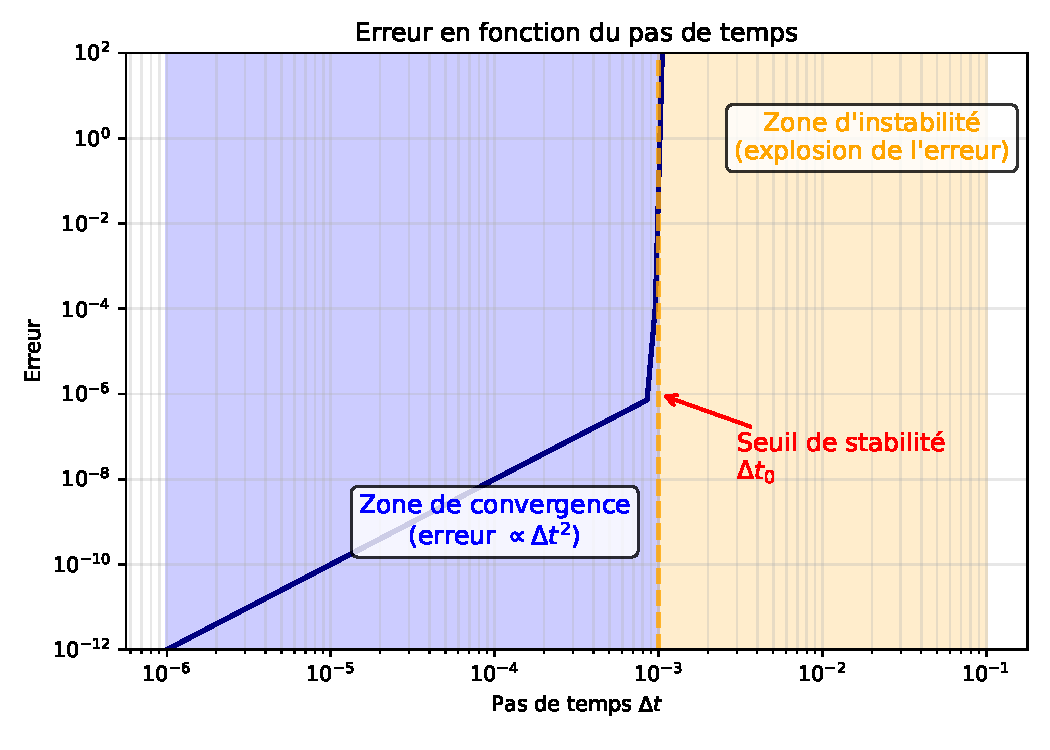
\includegraphics[width=0.8\textwidth]{media/3_/2_/exemple_satabilite.pdf}
    \caption{Illustration du comportement attendu de l'erreur d'un schéma d'ordre deux dont le seuil d'instabilité est $\Delta t > 10^{-1}$.}
    \label{fig:stabilite_schema}
\end{figure}

\begin{definition}[Stabilité d'un schéma numérique]
Un schéma numérique $\bigl(u^n\bigr)_{n\in\mathbb{N}} \in (\mathbb{R}^d)^{\mathbb{N}}$ est dit stable si la norme de la solution ne croît pas d’un pas de temps à l’autre :
\begin{align}
    \Vert u^{n+1} \Vert \leq \Vert u^n \Vert.
\end{align}
En pratique, cette condition est satisfaite lorsque $\Delta t$ reste inférieur à un seuil $\Delta t_0$ dépendant du problème et du schéma.
\end{definition}

La stabilité d’un schéma dépend directement du spectre de l’opérateur $A$ dans l’équation différentielle (cf. \eqref{def:def_ODE}).  
Lorsque $A$ possède des valeurs propres à grande partie réelle négative, les méthodes explicites imposent des pas $\Delta t$ extrêmement petits pour rester stables.  
Dans ce cas, le problème est qualifié de \emph{raide}.

\begin{definition}[Problème raide]
Un système dynamique
\begin{align}
    \frac{\text d u}{\text d t} = A(u,t), \qquad u(t)\in\mathbb{R}^d
\end{align}
est dit \emph{raide} si la jacobienne $J_A$ admet des valeurs propres très négatives en valeur absolue, entraînant une condition de stabilité tellement restrictive que les méthodes explicites deviennent inutilisables en pratique.
\end{definition}

Pour analyser la stabilité d’un schéma, on utilise la notion de \emph{fonction de stabilité}, introduite à partir de l’équation test linéaire $u'=\lambda u$.

\begin{definition}[Fonction de stabilité]
Pour un schéma numérique appliqué à l’équation $u'=\lambda u$, on définit l’indice spectral $z=\lambda \Delta t$ et une fonction $S(z)$ telle que
\[
U^{n+1} = S(z)\,U^n.
\]
Le schéma est stable pour un pas $\Delta t$ donné si et seulement si
\begin{align}
    |S(z)| \leq 1.
\end{align}
\end{definition}

\begin{exemple}[Équation de Dahlquist]
Considérons
\begin{align}
    u'(t) &= -\lambda u(t), \quad \lambda>0, \\
    u(0) &= u_0,
\end{align}
dont la solution exacte est $u(t)=u_0 e^{-\lambda t}$.

\textbf{Raideur.}  
Lorsque $\lambda$ est grand, la décroissance est très rapide.  
Un schéma explicite impose alors un pas $\Delta t$ extrêmement petit pour rester stable : le problème est dit raide car les explicites échouent par instabilité.

\textbf{Fonction de stabilité.}  
On pose $z=\lambda \Delta t$ et on calcule $S(z)$ :
\begin{itemize}
    \item \emph{Euler explicite :} $U^{n+1}=(1-z)U^n \Rightarrow S(z)=1-z$.  
          Stabilité $\iff 0\leq z\leq 2$, soit $\Delta t \leq 2/\lambda$.  
          Pour $\lambda\gg 1$, la contrainte est prohibitive.
    \item \emph{Euler implicite :} $U^{n+1}=\tfrac{1}{1+z}U^n \Rightarrow S(z)=\tfrac{1}{1+z}$.  
          Ici $|S(z)|\leq 1$ pour tout $z\geq 0$ : aucune restriction sévère, même pour $\lambda$ très grand.
\end{itemize}

Cet exemple illustre la notion de raideur : un problème est dit raide lorsque les méthodes explicites deviennent inutilisables à cause de la contrainte de stabilité, alors qu’un implicite reste stable.
\end{exemple}

Pour aller plus loin, on peut introduire des notions plus fines (A-stabilité, L-stabilité), développées par exemple dans \cite{HairerAndWanner1}.


% \subsection{Stabilité et raideur}\label{par:stabilite_edo}
% Un schéma numérique d'ordre $p$ converge asymptotiquement en $O(\Delta t^p)$ vers la solution exacte de l'EDO lorsque $\Delta t$ est assez petit.
% Cependant, cette convergence n'est possible que si le schéma est \textbf{stable}.
% L'instabilité d'un schéma désigne la divergence de la solution numérique. 
% En pratique, au-delà d'un pas de temps critique $\Delta t_0$, 
% la norme de la solution numérique $\Vert u^n \Vert$ tend vers l'infini\footnote{Phénomène communément appelé "explosion" de la solution numérique.} (voir \ref{fig:stabilite_schema}).
% Cela impose une respecter une contrainte de stabilité du type $\Delta t \leq \Delta t_0$ pour entre dans le régime asymptotique de convergence du schéma.
% Si ce seuil $\Delta t_0$ très faible, la résolution de l'EDO nécessite un grand nombre d'itérations $T_{\text{final}}/\Delta t$, augmentant le coût calculatoire. 
% Les schémas explicites sont généralement plus prompts aux instabilités que les méthodes implicites.
% \par
% Cette instabilité peut s'interpréter de deux manières complémentaires : d'un point de vue mathématique, le schéma se comporte comme une suite géométrique de raison $|r| > 1$ ; 
% d'un point de vue physique, le schéma introduit artificiellement de l'énergie dans le système à chaque itération.
% \begin{figure}[htbp]
%     \centering
%     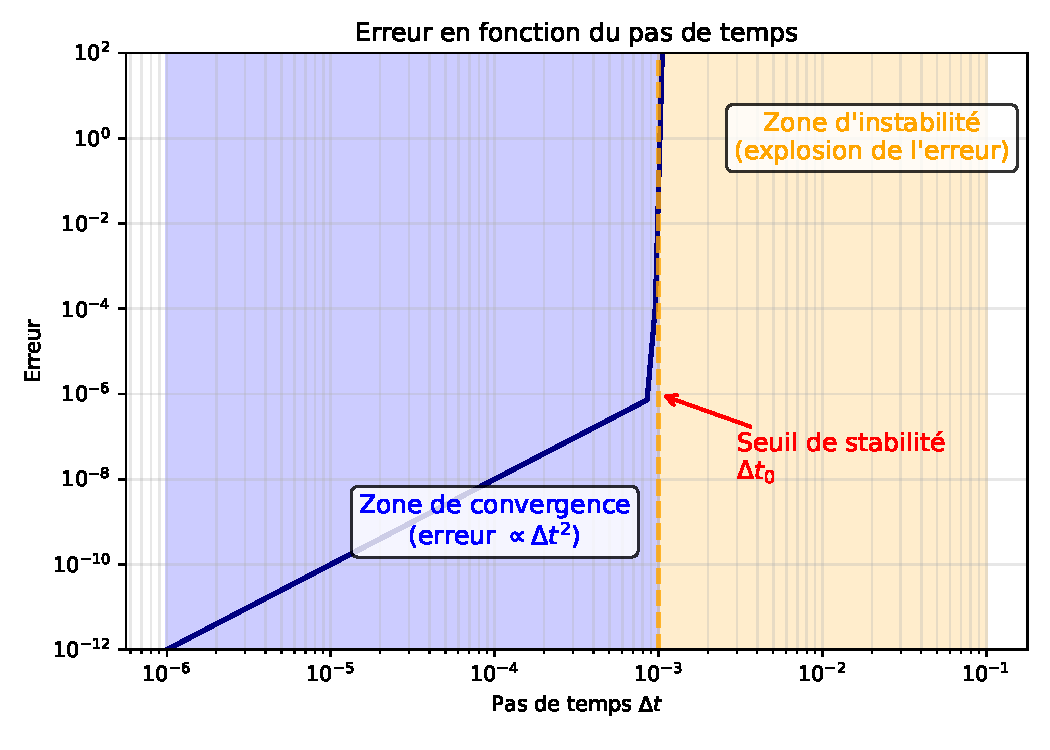
\includegraphics[width=0.8\textwidth]{media/3_/2_/exemple_satabilite.pdf}
%     \caption{Illustration du comportement attendu de l'erreur d'un schéma d'ordre deux dont le seuil d'instabilité serait $\Delta t > 10^{-1}$.}
%     \label{fig:stabilite_schema}
% \end{figure}
% \begin{definition}[Stabilité d'un schéma numérique]
% Un schéma numérique $\bigl(u^n\bigr)_{n\in\mathbb{N}} \in (\mathbb{R}^d)^{\mathbb{N}}$ est dit stable si la norme de la solution ne croît pas au fil des itérations, c’est-à-dire si
% \begin{align}
%     \Vert u^{n+1} \Vert \leq \Vert u^n \Vert.
% \end{align}
% En pratique, cette condition n'est satisfaite que si le pas de temps $\Delta t$ reste inférieur à un seuil $\Delta t_0$ dépendant à la fois du problème et du schéma utilisé.
% \end{definition}

% La stabilité d’un schéma dépend fortement du spectre de l’opérateur $A$ apparaissant dans l’équation différentielle (cf. \eqref{def:def_ODE}).  
% Lorsque certaines valeurs propres de $A$ sont très grandes en valeur absolue et négatives, les méthodes explicites deviennent inadaptées : le problème est dit \emph{raide}.

% \begin{definition}[Problème raide]
% Un système dynamique
% \begin{align}
%     \frac{\text d u}{\text{d}t} = A(u,t), \qquad u(t)\in\mathbb{R}^d
% \end{align}
% est dit \emph{raide} si la jacobienne $J_A$ possède des valeurs propres négatives de grande amplitude, imposant des échelles de temps très différentes.  
% Dans ce cas, la condition de stabilité des méthodes explicites devient tellement restrictive qu’elles sont inutilisables en pratique.
% \end{definition}

% La stabilité d’un schéma se caractérise de façon pratique à l’aide de la notion de fonction de stabilité.  
% Pour une équation linéaire $u'=\lambda u$, on définit l’indice spectral $z=\lambda \Delta t$ et une fonction $S$ telle que
% \[
% U^{n+1} = S(z)\,U^n.
% \]

% \begin{definition}[Fonction de stabilité]
% Un schéma numérique est stable pour un pas de temps $\Delta t$ donné si et seulement si
% \begin{align}
%     |S(z)| \leq 1 \qquad \text{avec } z=\lambda\Delta t.
% \end{align}
% \end{definition}

% \begin{exemple}[Équation de Dahlquist]
% Considérons l’équation test
% \begin{align}
%     u'(t) &= -\lambda u(t), \quad \lambda>0, \\
%     u(0) &= u_0.
% \end{align}
% Sa solution exacte est $u(t)=u_0 e^{-\lambda t}$.

% \medskip
% \textbf{Raideur.}  
% Si $\lambda$ est grand, la solution décroît très vite. Un schéma explicite impose alors un pas $\Delta t$ extrêmement petit pour rester stable : le problème est raide, au sens où l’explicite échoue par instabilité.

% \medskip
% \textbf{Fonction de stabilité.}
% \begin{itemize}
%     \item \emph{Euler explicite :} $U^{n+1}=(1-z)U^n \Rightarrow S(z)=1-z$.  
%         Stabilité $\iff 0\leq z\leq 2$, soit $\Delta t \leq 2/\lambda$. Pour $\lambda\gg 1$, cette contrainte est prohibitive.

%     \item \emph{Euler implicite :} $U^{n+1}=\tfrac{1}{1+z}U^n \Rightarrow S(z)=\tfrac{1}{1+z}$.  
%         Ici $|S(z)|\leq 1$ pour tout $z\geq 0$, donc aucune restriction sévère même pour des $\lambda$ très grands.
% \end{itemize}

% Cet exemple illustre la notion de raideur : la stabilité interdit l’usage d’un explicite, tandis qu’un implicite reste stable.
% \end{exemple}

% Pour aller plus loin, on introduit des notions plus fines comme la A-stabilité (stabilité pour tout $z$ à partie réelle négative) ou la L-stabilité (amortissement des modes très raides). Ces définitions, classiques en analyse numérique, sont détaillées par exemple dans \cite{HairerAndWanner1}.

% \begin{definition}[Stabilité d'un schéma numérique]
%     Un schéma numérique $\bigl( u^n \bigr)_{n \in \mathbb{N}} \in\bigl(\mathbb{R}^d \bigr)^{\mathbb{N}}$ est stable si et seulement si :
%     \begin{align}
%         \Vert u^{n+1} \Vert \leq \Vert u^n \Vert.
%     \end{align}
%     Cette condition est souvent vérifiée à la condition que le pas de discrétisation $\Delta t$ n'excède pas un seuil de stabilité $\Delta_0$ fonction de l'ODE et le schéma d'intégration.
% \end{definition}
% La stabilité d'une méthode d'intégration d'EDO dépend entre autres de l'opérateur intervenant dans l'équation (le $A$ dans l'équation \ref{def:def_ODE}).
% Un opérateur tendant à poser des problèmes de stabilité est dit raide.
% \begin{definition}[Problème raide]
%     Un système dynamique, est dit raide si les méthodes explicites ne sont pas adaptées à sa résolution.
%     En termes plus mathématiques le système:
%     \begin{align}
%     \frac{\text d u}{\text{d}t} = A(u,t), \quad u(t) \in \mathbb{R}^d, \forall t\geq 0.
%     \end{align}
%     est dit raide si la jacobienne de $A$, $J_A$ possède des valeurs propres négatives de grande amplitudes devant les autres valeurs propres.
%     Si tel est le cas, plusieurs relaxations sont mises en jeu mais chacune avec des temps caractéristiques d'ordres de grandeur différents.
%     Pour les méthodes explicites, si le pas de temps n'est pas assez petit, la relaxation rapide est mal résolue et
%     impose un gradient fort trop longtemps (le gradient devrait s'atténuer, mais à une échelle trop rapide pour être captée pour le pas de temps du schéma) ce qui 
%     déstabilise la méthode.
% \end{definition}
% En simplifiant, si un opérateur est raide, il impose une condition de stabilité très restrictive aux méthodes explicites et 
% force à choisir des méthodes implicites\footnote{La réalité est plus nuancée, nous le verrons.}.

% La limite de stabilité dépend du spectre de l'opérateur intervenant dans l'équation différentielle. 
% Pour une équation linéaire, cette limite dépend de chaque valeur propre de l'opérateur et peut être exprimé grâce à une \textit{fonction de stabilisé} fonction 
% d'un \textit{indice spectral}, produit de la valeur propre par la pas de temps: $z = \lambda \, \Delta t$.
% \begin{definition}[Fonction de stabilité]
%     Pour un schéma numérique donné, la fonction de stabilité $S$ est une fonction qui vérifie :
%     \begin{align}
%         (\text{Le schéma est stabile pour le pas de temps }\Delta t \iff \vert S(z) \vert < 1.)
%     \end{align}
% \end{definition}


% \begin{exemple}[Équation de Dahlquist]
% On considère l’équation test
% \begin{align}
%     \frac{\text d u}{\text d t} &= - \lambda u, \quad \lambda > 0, \\
%     u(0) &= u_0.
% \end{align}
% La solution exacte est $u(t) = u_0 e^{-\lambda t}$.

% \textbf{Raideur et stabilité.}
% Lorsque $\lambda$ est grand, la décroissance de la solution est très rapide.  
% Pour un schéma explicite, la stabilité impose en plus de prendre un pas $\Delta t$ extrêmement petit.  
% Autrement dit, la méthode explicite échoue par instabilité : c’est bien \emph{problème raide}.  
% Un problème est dit raide précisément quand les méthodes explicites deviennent inutilisables à cause de la condition de stabilité.

% \textbf{Fonction de stabilité.}
% On introduit l’indice spectral $z=\lambda \Delta t$ et la fonction de stabilité $S(z)$ définie par
% \[
% U^{n+1} = S(z)\,U^n.
% \]

% - \emph{Euler explicite :} $U^{n+1} = (1-z)U^n \;\Rightarrow\; S(z)=1-z$.  
% La condition $|S(z)|\leq 1$ impose $0 \leq z \leq 2$.  
% Donc si $\lambda$ est très grand, $\Delta t$ doit être minuscule : l’explicite devient inutilisable.

% - \emph{Euler implicite :} $U^{n+1} = \tfrac{1}{1+z} U^n \;\Rightarrow\; S(z)=\tfrac{1}{1+z}$.  
% On a $|S(z)|\leq 1$ pour tout $z \geq 0$, donc aucune contrainte de stabilité sévère, même si $\lambda$ est grand.

% Cet exemple montre comment la raideur se manifeste : l’explicite explose, l’implicite reste stable.
% \end{exemple}


% Il existe différents types de stabilité comme la A-stabilité (méthode stable indépendamment de la raideur du problème), la L-stabilité (schéma amortissant les hautes fréquences),
% par souci de concision cette partie s'achève ici mais ces notions sont développées par exemple dans \cite{HairerAndWanner1}.